\setcounter{step}{0}

\subsection{ Džadky }

\begin{ingredient}
  
      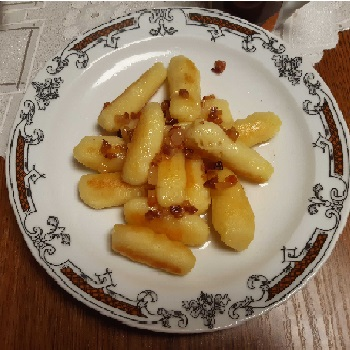
\includegraphics[height=5.5cm]{images/dzadky}
  
  \def\portions{  }
  \textbf{ {\normalsize Ingrediencie (4 porcie):} }

  \begin{main}
      \item 1kg zemiaky
      \item 350g hrubá múka
      \item 2KL soľ
      \item slanina
  \end{main}
  
\end{ingredient}
\begin{recipe}
\textbf{ {\normalsize Príprava:} }
\begin{enumerate}

  \item{Očistiť zemiaky, dať variť aby boli tesne zakryté vodou}
  \item{Zamiaky popučiť vo vode}
  \item{Pridať múku}
  \item{Nechať postáť, aby múka v horúcich zemiakoch napučala}
  \item{Vyvaľkať džadky}
  \item{Popražiť na panvici}
  \item{Posypať opraženou slaninkou}

\end{enumerate}
\end{recipe}

\begin{notes}
  
\end{notes}	
\clearpage
